\chapter{Einleitung}

Die Sprache des Menschen ist die natürlichste Art und Weise um miteinander zu kommunizieren. Durch die technische Entwicklung in den letzten Jahren kommen immer mehr Interaktionen zwischen Mensch und Maschine durch die Sprache zustande \cite{badshah2019deep}. Die Bezeichnung dafür sind die sogenannten intelligent personal assistants (IPAs) wie zum Beispiel Amazon Alexa, Apple Siri und Google Assistant. Google Home, Amazon Echo und Apple HomePod sind Home-Assistant Systeme, die primär Sprachsignale als Interaktionsmöglichkeit besitzen. Diese IPAs sind sehr stark verbreitet und auf vielen Geräten verfügbar \cite{speech_in_hci}.


\section{Was ist speech emotions recognition (SER)}
SER ist ein Forschungsgebiet, welches sich mit der Analyse von Audiosignalen in Form von Spektogrammen beschäftigt. In den letzten Jahren wurden in dem Gebiet von Spracherkennung signifikante Fortschritte gemacht. Die Audiosignale enthalten nicht nur die gesprochenen Wörter, sondern vielmehr auch den emotionalen Zustand des Sprechers \cite{badshah2019deep,speech_in_hci}. Das Ziel hierbei ist es durch verschiedene machine-learning Algorithmen das menschliche Befinden, die Gefühle und Emotionen aus den Audiosignalen zu extrahieren und somit den emotionalen Zustand des Sprechers zu erkennen. SER kann zum Beispiel als diagnostisches Werkzeug für Therapeuten verwendet werden. Eine weitere Einsatzmöglichkeit bietet SER bei Notrufzentralen, um die Ernsthaftigkeit der Situation des Anrufenden maschinell durch die Stimme erkennen zu können \cite{badshah2019deep}.

\section{Spektogramme}
Spektogramme spielen bei SER eine wichtige Rolle, denn sie dienen als Input. 
\begin{figure}
	\centering
	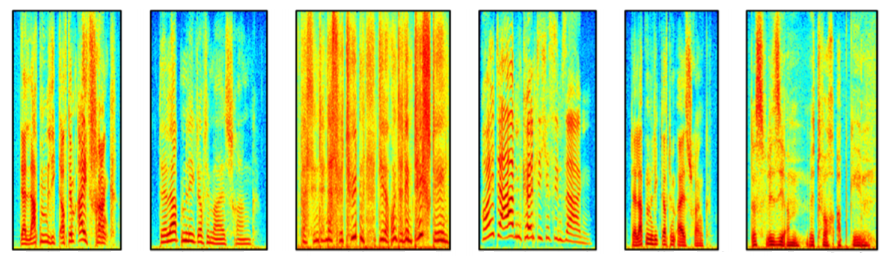
\includegraphics[width=1\textwidth]{images/spekto.PNG}
	\caption{\label{spektogram}Spektogramme für verschiedene Emotionen \cite{badshah2019deep}}
\end{figure}
\subsection{STFT und FFT}

%Bilder kann man natürlich auch in Arbeiten integrieren. Für Fotos und ähnliches %unterstützt PDF-\LaTeX{} direkt \verb|jpg| und \verb|png|, ansonsten empfiehlt es sich %Vektorgrafiken zu verwenden und diese als \verb|pdf| zu speichern. Sollte ein Bild %einmal zu viel weißen Raum um sich haben, so kann man mit dem Werkzeug \verb|pdfcrop| %das Bild automatisch ausschneiden

%\begin{figure}[ht]
%    \centering
%    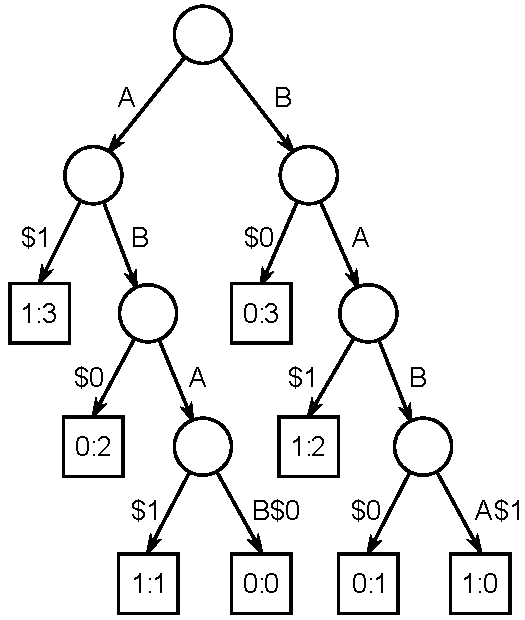
\includegraphics[width=.4\textwidth]{images/Suffix_tree_ABAB_BABA}
%    \caption{\label{anker}Bechreibung des Bilds}
%\end{figure}

%Mit Hilfe eines Labels kann man sich dann im Text auf diese Grafik (\ref{anker}) %beziehen. 

%\begin{figure}[ht]
%    \centering
%    \subfigure[Ein fettes u]{
%        
\includegraphics[width=0.2\linewidth]{images/a}
%        \label{subfigurebsp:a}
%    }
%    \hspace{1cm}
%    \subfigure[Ein dünneres u]{
%        
\includegraphics[width=0.2\linewidth]{images/b}
%        \label{subfigurebsp:b}
%    }
%    \caption{Die \emph{u}s aus der Wortmarke}
%\end{figure}

%Durch \verb|subfigure| lassen sich auch zwei kleine Bilder nebeneinander setzen. In %Abbildung \ref{subfigurebsp:a} ist ein fettes u auf der linken und in %\ref{subfigurebsp:b} ein dünneres auf der rechten Seite zu sehen.


%\subsection{Tabellen}

%Hier nur ein kurzes Beispiel, in jedem \LaTeX{} Buch finden sich gute Anleitungen zum %Erstellen von Tabellen.

%\begin{table}[h]
%    \centering
%    \begin{tabular}{|l|l|l|}
%        A & B & C \\
%        \hline
%        x & x & x \\
%        x & x & x
%    \end{tabular}
%\end{table}


%\subsection{Formeln}

%Mathematische Formeln lassen sich als Umgebung mit \verb|\begin{math}| und \verb|\end{math}| erzeugen, es gibt aber auch eine abgekürzte Schreibweise mit \verb|\( Formel \)| wobei die Formel dann im laufenden Text bleibt. Die kürzeste Form ist mit zwei \verb|$| um die Formel, z.B.~so Wasser ist H$_2$O.

%Mit der Schreibweise \verb|\[ Formel \]| wird die Formel mittig auf einer neuen Zeile gesetzt, z.B.

%\[y = x^2 \]

%Dies ist die Kurzform der Umgebung \verb|equation|, mit der die Gleichung auch nummeriert wird. 

%\begin{equation}
%    x_{1,2} = \frac{-b\pm\sqrt{b^2-4ac}}{2a}
%    \label{mitternachtsformel}
%\end{equation}

%Wenn wir z.B.~über die beliebte Mitternachtsformel (Gleichung \ref{mitternachtsformel}) schreiben wollen lässt sich diese also wie ein Bild referenzieren.



